%===============================================================================
% Illinois Rocstar definitions
%===============================================================================
%&pdfLaTeX
% !TEX encoding = UTF-8 Unicode
\documentclass[12pt]{article}
\usepackage[top=1in, bottom=1in, left=1in, right=1in]{geometry}
%\usepackage[cm]{fullpage}
\usepackage[colorlinks=true,linkcolor=Teal,citecolor=Black,urlcolor=Blue]{hyperref}
\usepackage{ifxetex}
\usepackage{url}
\ifxetex
%\usepackage{fontspec}
%\defaultfontfeatures{Mapping=tex-text,Scale=MatchLowercase}
%\setmainfont[Scale=.95]{Times}
\setmainfont[Mapping=tex-text, Scale=2.0]{STIXGeneral}
\else
\usepackage[T1]{fontenc}
\usepackage[utf8]{inputenc}
\usepackage{lmodern}
\fi
\usepackage{textcomp}
\usepackage{natbib}  % formatting for references
\usepackage{mdframed}
\usepackage{setspace}
%\usepackage{ulem}
%\usepackage{amssymb}
\usepackage{amsmath,amssymb}
\usepackage{graphicx}% Include figure files
\usepackage{longtable} % allow multipage tables
\usepackage{multirow}
\usepackage{psfrag,rotating,multirow,setspace,colordvi}
\usepackage{epstopdf}
\usepackage{dcolumn}% Align table columns on decimal point
\usepackage{bm}% bold math
%\usepackage{subfigure}
%\usepackage{caption}
\usepackage[font={sf,normalsize},format=plain,labelfont=bf]{caption}
\usepackage{subcaption}
\usepackage{float}
%\usepackage{babel}
\usepackage{makeidx}
%\usepackage[font=footnotesize,format=plain,labelfont=bf,font=doublespacing]{caption}
%\usepackage{overcite}
\usepackage{color}
\usepackage[usenames,dvipsnames,svgnames,table]{xcolor}
\definecolor{color18}{rgb}{0.5,0.5,0.5}

% ==================================================
% Track changes and commenting packages and commands
% ==================================================
\usepackage{todonotes}
\newcommand{\jek}[1]{\todo[inline,color=purple!40,caption={}]{#1}}
\newcommand{\mdb}[1]{\todo[inline,color=orange!40,caption={}]{#1}}
\newcommand{\mja}[1]{\todo[inline,color=blue!40,caption={}]{#1}}
\newcommand{\mtc}[1]{\todo[inline,color=red!40,caption={}]{#1}}
\newcommand{\sam}[1]{\todo[inline,color=green!40,caption={}]{#1}}
\newcommand{\rxi}[1]{\todo[inline,color=yellow!40,caption={}]{#1}}

%\usepackage[addedmarkup=bf,deletedmarkup=sout]{changes} %Final showing markup
\usepackage[final]{changes} %Final

\definechangesauthor[color=purple]{jek}
\newcommand{\jeka}[1]{\added[id=jek]{#1}}
\newcommand{\jekd}[1]{\deleted[id=jek]{#1}}
\newcommand{\jekr}[2]{\replaced[id=jek]{#1}{#2}}

\definechangesauthor[color=orange]{mdb}
\newcommand{\mdba}[1]{\added[id=mdb]{#1}}
\newcommand{\mdbd}[1]{\deleted[id=mdb]{#1}}
\newcommand{\mdbr}[2]{\replaced[id=mdb]{#1}{#2}}

\definechangesauthor[color=blue]{mja}
\newcommand{\mjaa}[1]{\added[id=mja]{#1}}
\newcommand{\mjad}[1]{\deleted[id=mja]{#1}}
\newcommand{\mjar}[2]{\replaced[id=mja]{#1}{#2}}

\definechangesauthor[color=red]{mtc}
\newcommand{\mtca}[1]{\added[id=mtc]{#1}}
\newcommand{\mtcd}[1]{\deleted[id=mtc]{#1}}
\newcommand{\mtcr}[2]{\replaced[id=mtc]{#1}{#2}}

\definechangesauthor[color=green]{sam}
\newcommand{\sama}[1]{\added[id=sam]{#1}}
\newcommand{\samd}[1]{\deleted[id=sam]{#1}}
\newcommand{\samr}[2]{\replaced[id=sam]{#1}{#2}}

\definechangesauthor[color=yellow]{rib}
\newcommand{\riba}[1]{\added[id=rib]{#1}}
\newcommand{\ribd}[1]{\deleted[id=rib]{#1}}
\newcommand{\ribr}[2]{\replaced[id=rib]{#1}{#2}}
% ==================================================


% ==================================================
% SI units package and special commands
% ==================================================
\usepackage{siunitx}
\newcommand{\SIper}{\SI[per-mode=symbol]}
% ==================================================


% ==================================================
% Special page formatting commands 
% ==================================================

% Shorten or lengthen page by one line (for orphan lines)
\newcommand{\longpage}{\enlargethispage{\baselineskip}}
\newcommand{\shortpage}{\enlargethispage{-\baselineskip}}

% Wrap text to end of line for artificial line break
% (Shift-Enter in Word) for figure placement
\newcommand{\startsquarepar}{%
    \par\begingroup \parfillskip 0pt \relax}
\newcommand{\stopsquarepar}{%
    \par\endgroup}
% ==================================================


\usepackage{wrapfig}
%\usepackage{epstopdf}
%\usepackage[rflt]{floatflt}
\usepackage{fancyhdr}
%\setlength{\headheight}{12pt}
\setlength{\headheight}{25pt}
\setlength{\headsep}{.4in}
\setlength{\textheight}{650pt}
\setlength{\parskip}{5pt}
\setlength{\parindent}{0pt}
%\setlength{\footskip}{.1in}
\renewcommand{\headrulewidth}{.5pt}
\renewcommand{\footrulewidth}{0pt}


\newcommand{\tab}{\hspace{5mm}}

\usepackage{enumerate}

% IR-specific stuff
\usepackage{sectsty}
\allsectionsfont{\bfseries\sffamily}
\newcommand{\irpart}[2]{\part{\textsf{#1}}}
\newcommand{\irpara}[2]{\paragraph{\textsf{#1}}}
\newcommand{\irspara}[2]{\subparagraph{\textsf{#1}}}
\newcommand{\irparanonum}[2]{\paragraph*{\textsf{#1}}}
\newcommand{\irsection}[2]{\section{\textsf{#1}}\label{#2}}
\newcommand{\irsectionnonum}[2]{\section*{\textsf{#1}}\label{#2}}
\newcommand{\irssection}[2]{\subsection{\textsf{#1}}\label{#2}}
\newcommand{\irssectionnonum}[2]{\subsection*{\textsf{#1}}\label{#2}}
\newcommand{\irsssection}[2]{\subsubsection{\textsf{#1}}\label{#2}}
\newcommand{\irsssectionnonum}[2]{\subsubsection*{\textsf{#1}}\label{#2}}
\newcommand{\irtitle}[1]{\title{\bf{\textsf{#1}}}}
\newcommand{\irauthor}[1]{\author{\textsf{#1}}}
\newcommand{\irdate}[1]{\textsf{\date{#1}}}
\newcommand{\irtoday}{\textsf{\today}}
\newcommand{\rocstar}{{\textit{Rocstar}}}
\newcommand{\software}[1]{\textit{#1}}
\newcommand{\irfilename}[1]{\texttt{\textsf{#1}}}
\newcommand{\irwebsite}[1]{\irfilename{\bf #1}}
\newcommand{\commandline}[1]{\texttt{> #1}}
\newcommand{\plusplus}[1]{#1{}\texttt{++}}
\newcommand{\plus}[1]{#1{}\texttt{+}}
\newcommand{\irref}[2]{\hyperref[#2]{#1~\ref{#2}}}
\newcommand{\ireq}[2]{\hyperref[#2]{#1~(\ref{#2})}}
\newcommand{\irrefexp}[3]{\hyperref[#3]{{#1}~{#2}}}
\newcommand{\hilight}[1]{\colorbox{yellow}{#1}}
\def\Dpartial#1#2{ \frac{\partial #1}{\partial #2} }
\def\Dparttwo#1#2{ \frac{\partial^2 #1 }{ \partial #2^2} }
\def\Dpartpart#1#2#3{ \frac{\partial^2 #1 }{ \partial #2 \partial #3} }
\def\Dnorm#1#2{ \frac{d #1 }{ d #2} }
\def\Dnormtwo#1#2{ \frac{d^2 #1 }{ d #2 ^2} }
\def\Dtotal#1#2{ \frac{D #1 }{ D #2} }


\newcommand{\cJ}{\mathcal{J}}
\newcommand{\cI}{\mathcal{I}}
\newcommand{\cM}{\mathcal{M}}
\newcommand{\cP}{\mathcal{P}}
\newcommand{\cN}{\mathcal{N}}
\newcommand{\cC}{\mathcal{C}}
\newcommand{\cG}{\mathcal{G}}

\newcommand{\bx}{\mathbf{x}}
\newcommand{\bn}{\mathbf{n}}

\newcommand{\hh}{{\hat{h}}}
\newcommand{\rh}{{\hat{r}}}

\newcommand{\vvC}{{\Vec{\Vec{c}}}}
\newcommand{\vF}{{\vec{F}}}
%\newcommand{\vf}{{\vec{f}}}
\newcommand{\vb}{{\vec{b}}}
\newcommand{\vq}{{\vec{q}}}
\newcommand{\vR}{{\vec{R}}}
\newcommand{\vqs}{{\vec{q}^{\,*}}}
\newcommand{\vqsT}{{\vec{q}^{\,*T}}}
\newcommand{\vs}{{\vec{s}}}


\newcommand{\bxi}{\boldsymbol{\xi}}


\newcommand{\bbK}{{\mathbb{K}}}
\newcommand{\bbS}{{\mathbb{S}}}
\newcommand{\bbP}{{\mathbb{P}}}
\newcommand{\bbI}{{\mathbb{I}}}
\newcommand{\bbA}{{\mathbb{A}}}
\newcommand{\bbB}{{\mathbb{B}}}
\newcommand{\pOmega}{{\partial\Omega}}

%\providecommand{\e}[1]{\ensuremath{\times 10^{#1}}}

\def\eps{\varepsilon}
\def\bx{\mathbf{x}}
\def\bk{\mathbf{k}}
\def\bkappa{\boldsymbol{\kappa}}


\def\bdash{\hbox{\drawline{4}{.5}\spacce{2}}}
\def\spacce#1{\hskip #1pt}
\def\drawline#1#2{\raise 2.5pt\vbox{\hrule width #1pt height #2pt}}
\def\dashed{\bdash\bdash\bdash\bdash\nobreak\ }
\def\solid{\drawline{24}{.5}\nobreak\ }
\renewcommand{\thefootnote}{\fnsymbol{footnote}}
\renewcommand{\thispagestyle}[1]{} % do nothing

%command to generate the header, put #1 at the right (document title) and #2 centered (release statement)
\newcommand{\irheader}[2]
{
  \pagestyle{fancy}
  \rhead{}
  \rfoot{}
  \chead{}
  %\cfoot{\color{color18}{\thepage{}}}
  \fancyhead[LO,L]{
\includegraphics[width=24pt]{../Figures/IRTriangles.png}\color{color18}\textsf{\space Illinois Rocstar LLC}}
  \fancyhead[RO,R]{\color{color18}{\textsf{#1}}}
  \fancyhead[CO,C]{\color{color18}{\textsf{#2}}}
  \fancyfoot[CO,C]{\color{color18}{\thepage{}}}
}

%Command to generate the copyright page
\newcommand{\ircopyright}[0]
{
  %\clearpage\null
  \vfill
%\pagesytle{empty}
  \begin{minipage}[b]{0.9\textwidth}
  \footnotesize\raggedright
  \setlength{\parskip}{0.5\baselineskip}
  Copyright \copyright\the\year\ Illinois Rocstar LLC\par
  \irwebsite{www.illinoisrocstar.com}
  \end{minipage}
  \vspace*{2\baselineskip}
  \cleardoublepage
}

\newcommand{\ircallout}[3]
{
  \begin{wrapfigure}{#1}{#2\textwidth}
        \vspace{-20pt}
        \centering
        \fbox{\parbox{#2\textwidth}{#3}}
        \vspace{-10pt}
  \end{wrapfigure}
}

\newcommand\todoin[2][]{\todo[inline, caption={2do}, #1]{
\begin{minipage}{\textwidth-4pt}#2\end{minipage}}}

\newcommand{\todoingreen}[1]{\todo[inline, color=green!40]{#1}}            



% add copyright command to /maketitle
\makeatletter
\g@addto@macro{\maketitle}{\ircopyright}
\makeatother

\makeindex
\usepackage{dirtree}

% ******************
%  CALLOUT BOX CONSTRUCT
% ******************
%
%\begin{wrapfigure}{r}{0.3\textwidth}
%        \vspace{-20pt}
%        \centering
%        \fbox{
%             \parbox{0.3\textwidth}{
%                  This is a test of a callout box. 
%                  It has several lines and even a paragraph.
%
%                  See here for the new paragraph. This paragraph
%                  no longer has a bulleted list.
%             }                      
%        }
%        \vspace{-10pt}
%\end{wrapfigure}


%------------------------------------------------------------------
% Includeed Packages
%------------------------------------------------------------------
\usepackage{enumitem}
\usepackage{fancybox}
\usepackage{threeparttable}
\usepackage{url}
\usepackage{pdfpages}
\usepackage{multicol}
\usepackage{pgfplots}
\usepackage{etoolbox}
\usepackage{alphalph}
\usepackage{fancyvrb}
\usepackage{rotating}

%------------------------------------------------------------------
% New Commands: Program names
%------------------------------------------------------------------
%\newcommand{\myhline}{\arrayrulecolor{teal}\hline}

\newcommand{\Rocstar}{\software{Rocstar}}
\newcommand{\Rocburn}{\software{Rocburn\_PY}}

\newcommand{\midHeader}{}
\newcommand{\rightHeader}{\Rocburn\ Developer Guide}
\newcommand{\ir}{Illinois Rocstar LLC}

\DeclareSIUnit\calorie{cal}

%------------------------------------------------------------------
% Boolean to easily compile GUI and non-GUI relevant documentation (etoolbox)
%------------------------------------------------------------------
%\newbool{GUI}
%\booltrue{GUI}
%\boolfalse{GUI}

%\ifbool{GUI}
%
%

%------------------------------------------------------------------
%  These two lines will number figures and tables as #1.#2, where #1
%  number of chapter and #2 is the figure or table number within the chapter
%------------------------------------------------------------------
\renewcommand{\thefigure}{\thesection.\arabic{figure}}
\renewcommand{\thetable}{\thesection.\arabic{table}}
\renewcommand{\theequation}{\thesection.\arabic{equation}}
\renewcommand{\thefootnote}{\emph{\alphalph{\value{footnote}}}}
\newcommand\gauss[2]{1/(#2*sqrt(2*pi))*exp(-((x-#1)^2)/(2*#2^2))}

%==================================================================
% Document build
%==================================================================
\begin{document}
\setcounter{secnumdepth}{5}
\setcounter{tocdepth}{4}

\begin{figure}
  \centering
  
\includegraphics[height=3.in]{../Figures/IR_Logo.png}
\end{figure}
%-----------------------------------------------
\irtitle{\rightHeader}

\date{\textsf{\today}}

\pagestyle{empty}
\maketitle

%header and footer
\irheader{\rightHeader}{\midHeader}

\irsectionnonum{License}{lic}

The \Rocburn\ module of \Rocstar\ as well as its source, executables, and this document are the property of Illinois Rocstar LLC. Licensing and support of the software package, including full source access for government, industrial, and academic partners, are arranged on an individual basis. Please contact Illinois Rocstar at 
\begin{itemize}
  \item {\irwebsite{tech@illinoisrocstar.com}}
  \item {\irwebsite{sales@illinoisrocstar.com}}
\end{itemize}
for support and licensing.

\newpage

\setcounter{page}{1}
\pagestyle{plain}


%header and footer
\irheader{\rightHeader}{\midHeader}
\tableofcontents

\newpage

\setcounter{figure}{0}
\setcounter{table}{0}
\setcounter{equation}{0}

\irsection{Introduction}{Intro}

\Rocburn\ is defined by one-dimensional physics, appropriate for a homogeneous propellant, and it is assumed that its parameters can be chosen to represent the heterogeneous case in some fashion. The physics that is not accounted for in any plausible way in this strategy includes the non-planar surface regression and the diffusion flames in the combustion field. \Rocburn\ is a numerical module inside \Rocstar\ that simulates the thermal transient effects in the wall-normal direction of a homogeneous medium found in solid propellant rocket motors (e.g., insulated walls, propellant, nozzle, etc.). The time-dependent temperature in the solid is computed using a one-dimensional model that takes into account a temperature gradient normal to (only) the burning surface. Thus, the solid is essentially treated as a semi-infinite solid, and the unsteady heat equation is solved in the wall-normal direction. The \Rocburn\ table feature is created by averaging the solid phase heat conduction over a plane that is parallel to the mean surface, accounting for rotational terms that arise due to the uneven surface. Boundary conditions are applied at the propellant surface and include, most importantly, the heat flux from the combustion field. This heat flux is not modeled but is contained in a universal lookup generated by another module in \Rocstar. Information about combustion and ignition of solid propellants is available elsewhere [\cite{Ibiricu:1975,Blomshield:1997,Ward:1998,Brewster:2000,Chen:2002,Jackson:2002,Massa:2002,Massa:2004,Massa:2005}].
\setcounter{figure}{0}
\setcounter{table}{0}
\setcounter{equation}{0}

\irsection{Combustion and Ignition at the Propellant Surface}{Ibiricu}

Before presenting the theory behind the \Rocburn\ implementation, this section discusses the ideas of propellant combustion and ignition more broadly. The thermal transient theory inside \Rocburn\ is abstract, so presentation of this broader picture will help to concretize the physical phenomena taking place in the different regions, each modeled in its own way. The following figure and associated description are taken directly from [\cite{Ibiricu:1975}].

\begin{figure}[ht]
\centering
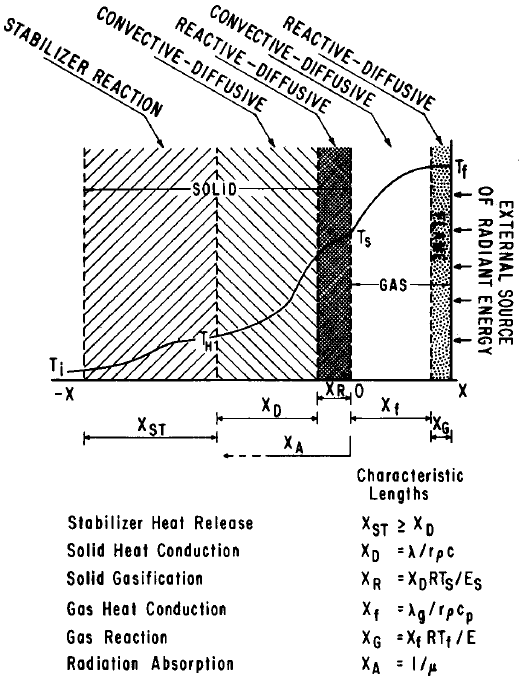
\includegraphics[width=0.5\textwidth]{../Figures/IbiricuCombustionModel.png}
\caption{Schematic illustration of combustion model from [\cite{Ibiricu:1975}]. Variable descriptions: solid thermal conductivity, $\lambda$; burn rate, $r$; density, $\rho$; solid heat capacity per unit mass, $c$; universal gas constant, $R$; temperature of solid surface, $T_s$; activation energy for solid phase reaction, $E_s$; gas thermal conductivity, $\lambda_g$; gas specific heat at constant pressure, $c_p$; flame temperature, $T_f$; activation energy for gas phase reaction, $E$; and absorption coefficient for solid, $\mu$.}
\label{fig:ibiricu}
\end{figure}

\begin{quote}
The combustion model is illustrated schematically in \irref{Figure}{fig:ibiricu}. The solid phase occupies the region $x < 0$ and the gas phase the region $x > 0$. Externally provided radiation is incident on the propellant from the gas. The temperature profile has been drawn for the unperturbed state of zero radiant flux. Allowance is made for gaseous and solid reactions, each being presumed to have activation energies
sufficiently high for reactive--diffusive and convective--diffusive zones to be identifiable [\cite{Williams:1973}]. In addition, a stabilizer reaction zone is included for propellants containing stabilizers that react exothermically at low temperatures [\cite{Huggett:1960,Kovalskii:1967}]. Regression rates are assumed to be controlled by the gaseous or solid reaction, or by a combination thereof, but not by the stabilizer reaction, whose effect is treated purely energetically.

Although it may not be apparent, the model encompasses conventional views of double-base propellant combustion [\cite{Huggett:1960}]. The convective--diffusive zone in the gas may represent the ``dark zone,'' and the reactive--diffusive zone in the solid is a combination of the subsurface and ``fizz'' reaction zones of the classical description. Placement of the surface on the hot side of this last zone, and calling it the ``solid reaction zone'' are merely conventions ... Experimental demarkation of a boundary between subsurface and fizz zones is inconclusive, and two-phase flow analyses needed in attempting to resolve the issue are very difficult. If the demarkation can be achieved, then a boundary temperature can be identified which conventionally has been called the ``surface temperature'' and which lies below the $T_s$ of \irref{Figure}{fig:ibiricu} when the reactive--diffusive zone of the solid encompasses the fizz zone. Since rates of fizz-zone reactions may be expected to depend on pressure, there should be no hesitance to assign pressure dependence to rates in the present ``solid reaction zone.'' The model is capable of retaining or excluding the break in the temperature curve shown at $x=0$.  [\cite{Ibiricu:1975}]
\end{quote}
\setcounter{figure}{0}
\setcounter{table}{0}
\setcounter{equation}{0}

\irsection{Review of Thermal Transient Theory Inside \Rocburn}{Theory}

The equation that governs the unsteady heat conduction in a homogeneous medium with a surface regressing normal to itself is given by

\begin{equation}
\rho_c c_p \left( {\partial T \over \partial t} + r_b {\partial T \over \partial x} \right)
 = \lambda_c {\partial^2 T \over \partial x^2}.
\label{eq:sld}
\end{equation}

Here $x$ is the distance normal from the surface with range $-x_{\rm end} < x < 0$, $r_b$ is the speed of the regressing surface, $T$ is the temperature, and $t$ is the time. The material properties $\lambda_c$, $\rho_c$, and $c_p$ are the thermal conductivity, density, and specific heat of the solid, respectively.

The appropriate boundary condition at $-x_{\rm end}$ then becomes

\begin{equation}
T(-x_{\rm end}) = T_\infty.
\label{eq:bc1}
\end{equation}

where $T_\infty$ is the supply (or ambient) temperature. The boundary condition at $x = 0$ may depend on if the expression is evaluated from the solid phase side ($0^-$) or the gas phase side ($0^+$) of the surface. For the convective--diffusion zone at the surface,

\begin{equation}
T(0^-)=T(0^+)\equiv T_s.
\label{eq:bc2}
\end{equation}

where $T_s$ is the surface temperature. The derivative with respect to $x$, evaluated from the solid phase side ($0^-$), is given by

\begin{equation}
{\partial T \over \partial x}(0^-) = g(T_s,T_g)
\label{eq:bc3}
\end{equation}

The flux function $g(T_s,T_g)$ is the heat flux from the gas phase to the solid phase surface where $T_g$ is the gas phase temperature. As might be implied, the heat flux depends on the surface temperature of the solid as well as the gas phase ``fluid'' lying above the surface. The actual form of the flux $g$ depends on whether the solid is a propellant, a no-slip wall, or an ablating wall. If the solid is a propellant, the form of $g$ also differs for times before and after ignition.
\irssection{Regression Speed}{rb}

For a moving surface the regression speed $r_b$ can be specified by one of two forms, as given in \ireq{eqs}{eq:pyro1} and \textcolor{teal}{(\ref{eq:pyro2})}, respectively. Trivially $r_b$ is zero if the surface is not regressing. A simple expression for $r_b$ can be defined by an experimentally determined power law for burning, 

\begin{equation}
r_b = A_p \left( \frac{P}{P_{\rm ref}} \right)^{n_p} 
\label{eq:pyro1}
\end{equation}

where $A_p$ is the steady state regression speed at reference pressure $P_{\rm ref}$, $n_p$ is the pressure exponent, and $P$ is the input pressure from the chamber, and $A_p$ and $n_p$ are empirical fits to data. Alternatively $r_b$  can be defined by a one-step Arrhenius pyrolysis model,

\begin{equation}
r_b = A_c \exp\left[ -\frac{E_c}{R_u T_s} \right] 
\label{eq:pyro2}
\end{equation}

where $A_c$ is the exponential prefactor, $E_c$ is the pyrolysis activation energy for the solid (condensed) phase, $R_u$ is the universal gas constant, and $T_s$ is the surface temperature.
\irssection{Heat Flux to the Surface}{g}

As discussed above, the actual form of the flux $g(T_s,T_g)$ depends on whether the solid is a propellant, a no-slip wall, or an ablating wall. If the solid is a propellant, the form of $g$ also differs for times before and after ignition.

\irsssection{Pre-Ignition Phase Along Propellant Surfaces}{PreIgnit}

If the temperature is lower than the ignition temperature, then no mass flux is injected at the propellant surface, and a turbulent boundary layer separates the inviscid field from the propellant surface. Because of this situation, it is assumed that the turbulent boundary layer along the propellant surface is not resolved numerically, and the flux to the (non-ignited) propellant surface is  approximated by integrating the Euler equations down to the surface. In such case $g(\cdots)$ is calculated as

\begin{equation}
g(T_s,T_g) = \frac{h (T_g - T_s)}{\lambda_c}.
\label{eq:qc}
\end{equation}

The film coefficient, $h$, is expressed in terms of the Stanton number {\sf St}, 

\begin{equation}
h = (U_\infty\rho_g c_p){\sf St}
\label{eq:hfilmcoeff}
\end{equation}

where $U_\infty$ is the free-stream velocity and $\rho_g$ is the density of the gas. For the boundary layer with constant free-stream velocity and wall temperature, the Stanton number is given by the Prandtl number {\sf Pr} and the Reynolds number {\sf Re}:

\begin{equation}
{\sf St} = 0.0287({\sf Pr})^{-2/5}({\sf Re}_{x})^{-1/5}.
\label{eq:stnum}
\end{equation}

Note that here, the Reynolds number is based on the streamwise coordinate $x$. Expanding these definitions gives the following expression for the film coefficient.

\begin{equation}
h=0.0287\rho_g U_\infty c_p\left(x\rho_g U_\infty\mu_g c_p^2\over \lambda_g^2\right)^{-1/5}
\label{eq:hfilmcoefffull}
\end{equation}

where $\lambda_g$ is the thermal conductivity of the gas and $\mu_g$ is the viscosity. Such a form is assumed valid for the general case in which both the wall temperature and free-stream velocity vary in $x$ and in time, using the numerically evaluated outer edge solution as the free-stream temperature and velocity. Finally, note that

\begin{equation}
{\partial g \over \partial T_s} = -{h \over \lambda_c}
\label{eq:qcprime}
\end{equation}

where $\lambda_c$ is the thermal conductivity of the solid as before.

\irsssection{Post-Ignition Phase Along Propellant Surfaces}{PostIgnit}

When the surface temperature reaches the ignition value, the surface cell is switched from a non-ignition surface to a burning cell,\footnote{That is, it is assumed that the transition events from ignition to complete combustion occur on a time scale that is too small to resolve numerically, and so the ignition event is treated as a on/off switch.} and the heat flux to the surface is evaluated by integrating the steady state convection--diffusion--reaction equations for the gas phase. Activation energy asymptotic theory is used to relate the flame temperature $T_\star$ to the surface temperature.

\begin{equation}
\frac{1}{2}\frac{E_g}{R_u} \left[ \frac{1}{T_\star^0} - \frac{1}{T_\star} \right]=
\frac{E_c}{R_u} \left[ \frac{1}{T_s^0} - \frac{1}{T_s} \right]
\label{eq:tstar}
\end{equation}

where the superscript zero ($i^0$) indicates the steady state values and the subscript star ($i_\star$) are the values at the outflow plane. Therefore $T_\star^0$ is the steady flame temperature, and the steady state surface temperature $T_s^0$ is taken by comparing the pyrolysis law in \ireq{eq}{eq:pyro2} to the experimental burn power law in \ireq{eq}{eq:pyro1}. As before with \ireq{eq}{eq:pyro2}, $E_c/R_u$ is the scaled activation energy for solid phase, and likewise $E_g/R_u$ is the scaled activation energy for gas phase (i.e., temperatures).

Once the relationship between flame temperature and surface temperature has been established,
the integration of the convection--diffusion--reaction equations, together with the connection
boundary condition at the interface, yields the following expression for $g(\cdots)$.

\begin{equation}
g(T_s,T_g) = \frac{r_b}{\alpha_c} \left[ T_\star^0 - T_\infty +  T_s - T_\star \right]
\label{eq:gofT}
\end{equation}

where $\alpha_c$ is the thermal diffusivity of the solid: $\alpha_c = \lambda_c / (\rho_c c_p)$. (See \ireq{eq}{eq:sld}.) A result of activation energy asymptotic theory is that the injection temperature is equal to the flame temperature: $T_{\rm inject} = T_\star$. Finally, note that

\begin{equation}
\frac{\partial g}{\partial T_s} = \frac{E_c}{R_u}\frac{1}{T_s^2} g
 + \frac{r_b}{\alpha_c} \left[ 1 - 2 \frac{E_c}{E_g}\frac{T_\star^2}{T_s^2} \right].
\label{eq:dgdT}
\end{equation}

Recent improvements to \Rocburn\ now allow for a lookup table to compute the flux $g$ rather than using the descriptions given above. Note that the lookup table is \textit{propellant specific} and requires significantly more work. For this reason the approach discussed above is sufficient for most purposes. Enabling the lookup table function in the \Rocburn\ input file (\texttt{TABUSE~=~1}) is \textit{strongly} discouraged.

\irsssection{Non-Propellant Surfaces}{Nonprop}

For the case of a no-slip wall or an ablating surface, the assumption is that the turbulent boundary layer will be resolved with enough accuracy as to capture the local heat flux to the wall from the gas phase. The solid phase equation is as before.

\software{Rocflo} solves the compressible equations using an explicit time integrator. In particular, for the cell adjacent to the surface, the cell-centered temperature is updated as

\begin{equation}
T_1^{n+1}=T_1^n + \Delta t\, \mbox{RungeKutta\_RHS}(T_s^n,T_1^n,T_2^n)
\label{eq:temp}
\end{equation}

and will not be discussed in detail here.\footnote{In actuality \software{Rocflo} solves the conservative form of the equations, not the primitive form. \ireq{Eq}{eq:temp} is only used here for illustration purposes.}  

With $T_1^{n+1}$ known from the gas phase, the flux function $g$ can be written as

\begin{eqnarray}
g&=&\lambda_g {\partial T \over \partial x} \\
 &\approx&\lambda_g^{n+1} \left( {{T_1^{n+1}-T_s^{n+1}} \over \Delta x} \right),
\end{eqnarray}

where $\Delta x$ is the distance from $T_1^{n+1}$ to the surface, i.e., it is just half the cell height in the wall-normal direction. The expression for the gas phase thermal conductivity at the surface can be expanded to

\begin{equation}
\lambda_g^{n+1}=\lambda_g^n + \left({\partial \lambda_g \over \partial T_s}\right)^n
\left( T_s^{n+1}-T_s^n \right).
\end{equation}

Thus, the flux connection condition in \ireq{eq}{eq:bc3} at $x=0$ becomes

\begin{equation}
{\lambda_c \over 2 \Delta z} \left[ -3T_s^{n+1} + 4T_{1,c}^{n+1}-T_{2,c}^{n+1}\right]
{dz \over dx}=
\left[ \lambda_g^n + \left({\partial \lambda_g \over \partial T_s}\right)^n
\left( T_s^{n+1}-T_s^n \right) \right]
 \left( {{T_{1,g}^{n+1}-T_s^{n+1}} \over \Delta x} \right),
\label{eq:noburn}
\end{equation}

and the subscripts $c$ and $g$ denote values in the solid (condensed) phase and the gas phase, respectively. Note that the flux function $g$ is quadratic in $T_s^{n+1}$, so only the correct root need be selected.
\setcounter{figure}{0}
\setcounter{table}{0}
\setcounter{equation}{0}

\irsection{Numerical Solution of Unsteady Heat Conduction}{NumSol}

To solve for unsteady heat conduction in \ireq{eq}{eq:sld}, subject to the boundary conditions in \ireq{eqs}{eq:bc1} \textcolor{teal}{-- (\ref{eq:bc3})}, a computational grid is introduced with a cluster of points close to the surface $x=0$. The code uses either an exponential grid or a boundary layer type grid. In either case, let $z=z(x)$ be the mapping. Then \ireq{eq}{eq:sld} transforms to

\begin{equation}
\rho_c c_p \left( {\partial T\over\partial t} + r_b {\partial T \over \partial z} {dz \over dx} \right) 
= \lambda_c \left[ {\partial^2 T \over \partial z^2} \left({dz \over dx}\right)^2
+ {\partial T \over \partial z} {d^2 z \over dx^2} \right].
\end{equation}

The flux boundary condition becomes

\begin{equation}
{\partial T \over \partial z}{dz \over dx}\left(0^-\right) = g\left(T_s,T_g\right).
\end{equation}

The transformed unsteady heat equation for the interior points is solved numerically using a simple, first-order time integrator of the form

\begin{equation}
T^{n+1}=T^n~+~\Delta t\left[ 
\alpha_c \left( {\partial T \over \partial z} {d^2z \over dx^2}
+ {\partial^2 T \over \partial z^2} \left({dz \over dx}\right)^2 \right)
- r_b {\partial T \over \partial z} {dz \over dx} \right],
\label{eq:fotimeint}
\end{equation}

where $\alpha_c=\lambda_c/(\rho_c c_p)$ is the thermal diffusivity as before. A first-order time integrator is used because the timestep is typically small, and computational speed dictates that the integrator be fast. The spatial derivatives are computed using standard second-order central difference schemes. In all of test simulations, this approach was deemed sufficient.

The surface temperature at timestep $n+1$, i.e., $T_s^{n+1}$, is found from the flux boundary condition.
Note, however, that the equation is nonlinear in the surface temperature $T_s$. Since the timesteps are small, a full Newton method is not used; rather the $g$ function is expanded about the previous timestep of $T_s$ using Taylor's Theorem:

\begin{equation}
g(T_s^{n+1},T_g^{n+1})\approx g(T_s^n,T_g^n) +
\left. {\partial g \over \partial T_s}\right|_{T_s^n}\left(T_s^{n+1}-T_s^n\right).
\end{equation}

Then using a standard one-sided, second-order finite difference scheme, the updated surface temperature is expressed as

\begin{equation}
T_s^{n+1}=\frac{ 4T_2^{n+1} - T_3^{n+1} - {2 \Delta z \over dz/dx}g
 + {2 \Delta z \over dz/dx} {\partial g \over \partial T_s} T_s^{n}}
{3 + {2 \Delta z \over dz/dx} {\partial g \over \partial T_s} }.
\end{equation}

The value of $g(T_s^n)$ and $\partial g/\partial T_s(T_s^n)$, which is computed in the subroutine \texttt{GFUN} (\irref{Section}{Update}), depends on the specific conditions selected by the user; a more detailed discussion is presented in \irref{Section}{Input}.
\setcounter{figure}{0}
\setcounter{table}{0}
\setcounter{equation}{0}

\irsection{Physics Implementation in \Rocburn\ Source}{Code}

\Rocburn\ is a module within the larger multiphysics code \Rocstar. Its one-dimensional model is called a series of times, iterating over every surface point (or cell). The one-dimensional approach described above implies that each surface point is treated independently of the others. Specifically for the propellant surface, \ireq{eq}{eq:sld} is integrated for each point on the gas--solid interface. 

The burn update is invoked by the main flow solver for each surface point at each timestep of the unsteady simulation. The temperature outside the turbulent boundary layer and the film coefficient are passed as input from the main solver to the burn update module, which computes the burn rate and the temperature of the injected gas used in the fluid phase boundary conditions. Porous surface boundary conditions are imposed for $T_s > T_{\rm ignition}$ while solid surface boundary conditions are applied for $T_s < T_{\rm ignition}$. 

The unsteady heat conduction equation, \ireq{eq}{eq:sld}, is discretized using second-order, finite differences in the spatial directions and a first-order, forward difference scheme in time. The very thin temperature boundary layer associated with the heat wave traveling into the solid requires a stretched grid to properly resolve the heat flux at the surface. To preserve second-order spatial accuracy, a computational mapping is used. The von Neumann boundary condition at the fluid--solid interface is imposed by solving a discrete form of \ireq{eq}{eq:bc3}. The first derivative is discretized using a standard second-order, one-sided formula and the nonlinear function $g$ is expanded in a Taylor's series up to first order to obtain an explicit expression for the temperature at the surface, i.e., $T_s$. 

For non-propellant surfaces, the treatment is similar to that just described except that the flux condition \ireq{eq}{eq:bc3} is treated differently. In fact it can be shown that the numerical approximation leads to a quadratic function for the surface temperature, and the correct root must be taken. It is assumed, however, that, in the gas phase, the resolution is such that the heat flux can be adequately captured for time-accurate solutions.

As might be implied from above, the two main functions of \Rocburn\ are to pass information to the main solver upon initialization (e.g., temperature outside the turbulent boundary layer and the film coefficient) and then to update and compute the burn rate and heat flux as a function of time. The implementation is straightforward, and \Rocburn\ only has three main files and a limited number of subroutines. Information specific to the various files and subroutines are given in more detail below.

\begin{description}
\item[\irfilename{setup\_py.f90}]{Reads user parameters from input file, sets up the (internal \Rocburn) grid and timestep information, and reads the data from the table (if enabled)}
\item[\irfilename{init\_py.f90}]{Sets up the initial conditions for $t=0$ and determines if any cells are set to burning upon initialization}
\item[\irfilename{update\_py.f90}]{Updates the various temperatures and variables as functions of time, determines if new cells are burning (i.e., $T_s > T_{\rm ignition}$), and calculates the flux $g$}
\end{description}

\irssection{Problem Setup}{Setup}

\begin{Verbatim}[frame=single]
                              setup_py.f90

MODULE SETUP_PY

  USE data_py

CONTAINS

  SUBROUTINE get_time_step_1d(bp,rb,Toa,dt_max)
  SUBROUTINE burn_init_0d(bp,comm,IN_DIR,nx_read,To_read)
  SUBROUTINE read_properties(bp,IN_DIR)
  SUBROUTINE grid(bp)
  SUBROUTINE READTABLE(bp,IN_DIR)
  SUBROUTINE STEADYTEMP(bp,TIN,pIN,out,rb,g)
  SUBROUTINE CHECK_INPUT_RANGE(bp)
  SUBROUTINE burn_finalize_0d(bp)
\end{Verbatim}

\begin{description}
\item[\texttt{get\_time\_step\_1d(bp,rb,Toa,dt\_max)}]{\hfill \\ \vspace{-15pt}
\begin{itemize}  
\item{Variable \texttt{dt\_max = delt\_max}}
\end{itemize}
}

\item[\texttt{burn\_init\_0d(bp,comm,IN\_DIR,nx\_read,To\_read)}]{\hfill \\ \vspace{-15pt}
\begin{itemize} 
\item{Call \texttt{read\_properties} to read in the propellant thermophysical properties}
\item{Set the return values \texttt{nx\_read = numx} and \texttt{To\_read = To} that are read from input}
\item{Call \texttt{grid} to set up the computational grid}
\item{If a table is to be read from input, then call \texttt{readtable}}
\end{itemize}
}

\item[\texttt{read\_properties(bp,IN\_DIR)}]{\hfill \\ \vspace{-15pt}
\begin{itemize} 
\item{Read in all 29 required input parameters from \irfilename{RocburnPYControl.txt} and write them to the screen for verification}
\item{Note that the 29 parameters must be in the proper order and that the input file is named appropriately}
\item{Input parameters are discussed in detail in \irref{Section}{Input}}
\item{Call \texttt{CHECK\_INPUT\_RANGE} to verify input parameters}
\end{itemize}
}

\item[\texttt{grid(bp)}]{\hfill \\ \vspace{-15pt}
\begin{itemize}
\item{Variables \texttt{gridtype = igrid}, \texttt{numx = numx}, \texttt{beta = beta}, \texttt{xmax = xmax}, and \texttt{delz = 1 / (numx-1)}, which are all read from the input file}
\item{Set up $x$- and $z$-coordinate arrays}
\item{Set up first and second derivatives of $z$, i.e., $zx$ and $zxx$, respectively}
\item{Create either exponential or boundary layer grid, depending on \texttt{igrid} input parameter choice}
\item{Calculate maximum $\Delta t$ for time integration}
\item{Call \texttt{STEADYTEMP} to get appropriate state state temperature information}
\end{itemize}
}

\item[\texttt{READTABLE(bp,IN\_DIR)}]{\hfill \\ \vspace{-15pt}
\begin{itemize}
\item{If the table read option is enabled in the input file, read the name of the file with the table information, which is also specified in the input file}
\item{Allocate table fields and work fields}
\end{itemize}
}

\item[\texttt{STEADYTEMP(bp,TIN,pIN,out,rb,g)}]{\hfill \\ \vspace{-15pt}
\begin{itemize}
\item{Variable \texttt{To = To}, which is read from the input file}
\item{Call \texttt{polin2} (several times) to pass in information read from the table}
\item{Variable \texttt{out = g - (Tin - To)*rb / alfa}}
\end{itemize}
}

\item[\texttt{CHECK\_INPUT\_RANGE(bp)}]{\hfill \\ \vspace{-15pt}
\begin{itemize}
\item{Check that 14 selected parameters of the total 29 lie within the proper range}
\item{Input parameters and their associated ranges are discussed in detail in \irref{Section}{Input}}
\end{itemize}
}

\item[\texttt{burn\_finalize\_0d(bp)}]{\hfill \\ \vspace{-15pt}
\begin{itemize}
\item{Deallocate \texttt{bp} global array that contains data read from input}
\end{itemize}
}

\end{description}

\irssection{Parameter Initialization at \textit{t} = 0}{Init}

\begin{Verbatim}[frame=single]
                              init_py.f90

MODULE INIT_PY

  USE data_py

CONTAINS

  SUBROUTINE burn_get_film_coeff_1d(bp,p_coor,Ts,Teuler,P_in,Qc,Qcprime)
  SUBROUTINE burn_init_1d(bp,bflag,Pin,To,rhoc,p_coor,rb,Toa,fr,Tn,Tflame)    
\end{Verbatim}

\begin{description}

\item[\texttt{burn\_get\_film\_coeff\_1d(bp,p\_coor,Ts,Teuler,P\_in,Qc,Qcprime)}]{\hfill \\ \vspace{-15pt}
\begin{itemize}
\item{Variable \texttt{P = P\_in}}
\item{Variable \texttt{Te = min(Teuler,2*Tstar0)}, where  \texttt{Tstar0} is read from the input file (Note: \texttt{Teuler} is $T_g$ in \irref{Section}{Theory})}
	\begin{itemize}
		\item{Avoid Euler temperatures larger than twice the adiabatic flame temperature}
		\item{Note: ``This is a temporary hardwired fix. It should never affect the solution.''}
	\end{itemize}

\item{Review \texttt{ixsymm} parameter read from the input file, and if it is nonzero, the cell is already burning at $t=0$}

	\begin{itemize}

	\item{If \texttt{ixsymm.ge.1}, then...}
		\begin{itemize}
			\item{Variable \texttt{x\_surf = p\_coor(ixsymm)}, where \texttt{ixsymm} is 1, 2, or 3 for $x$, $y$, or $z$, respectively}
			\item{Calculate the film coefficient $h$ based on \ireq{eqs}{eq:hfilmcoeff} \textcolor{teal}{-- (\ref{eq:hfilmcoefffull})}}
			\item{Variable \texttt{front\_dist = x\_surf - x\_surf\_burn} where \texttt{x\_surf\_burn} is read from the input file}
			\item{Variable \texttt{try\_film} is determined from calculated $h$ (and other constants)}
		\end{itemize}

	\item{Else...}
		\begin{itemize}
			\item{Variable \texttt{try\_film = film\_cons}, which is read from the input file}
		\end{itemize}

	\end{itemize}

\item{Calculate the heat flux \texttt{Qc} and the derivative of the heat flux \texttt{Qcprime} (Note: The heat flux is specified by $g(T_s,T_g)$ in \irref{Section}{g})}
	\begin{itemize}
		\item{$Q_c$ (i.e., $g$) is given by \ireq{eq}{eq:qc} and cannot be negative, where the $\Delta T$ coefficient is the appropriate \texttt{try\_film}}
		\item{$Q_c^\prime$ (i.e., $g^\prime$) is given by \ireq{eq}{eq:qcprime}, using the appropriate \texttt{try\_film}}
	\end{itemize}

\end{itemize}
}

\item[\texttt{burn\_init\_1d(bp,bflag,Pin,To,rhoc,p\_coor,rb,Toa,fr,Tn,Tflame)}]{\hfill \\ \vspace{-15pt}
\begin{itemize}
\item{Review the \texttt{ixsymm} parameter read from the input file, and if it is nonzero, the cell is already burning at $t=0$}

	\begin{itemize}

	\item{If \texttt{ixsymm.ge.1}, then...}
		\begin{itemize}
			\item{Variable \texttt{x\_surf = p\_coor(ixsymm)}, where \texttt{ixsymm} is 1, 2, or 3 for $x$, $y$, or $z$, respectively}
			\item{If \texttt{x\_surf.le.x\_surf\_burn}, then burn flag \texttt{bflag = 1}; else \texttt{bflag = 0}}
		\end{itemize}

	\item{Else...}
		\begin{itemize}
			\item{Flag \texttt{bflag = 0}}
		\end{itemize}

	\end{itemize}
	
\item{Convert \texttt{P = Pin*pa2atm}}
\item{Calculate $T_s$ and $r_b$ given \texttt{To} and \texttt{P}}

	\begin{itemize}

	\item{If \texttt{bflag.ne.0}, then...}
		\begin{itemize}
			\item{If no table is read from input, then...}
				\begin{itemize}
					\item{Calculate \texttt{rb} using \ireq{eq}{eq:pyro1}}
					\item{\ireq{Eq}{eq:pyro2} is rearranged to solve for $T_s$}
					\item{Using value for \texttt{rb}, calculate \texttt{Ts} from rearranged \ireq{eq}{eq:pyro2}}
					\item{Variable \texttt{alp = alfac}, which is read from the input file}
				\end{itemize}
			
			\item{Else...}
				\begin{itemize}
					\item{Call \texttt{polin2} (several times) and pass in information read from the table}
				\end{itemize}
			
			\item{Variable \texttt{xcond = rb / alp}}
			\item{Variable \texttt{dtemp = Ts - To}}
			\item{Loop over all grid points and calculate variable \texttt{Tn} ($T^n$) at every grid point for use later with \ireq{eq}{eq:fotimeint}}
			\item{Variable \texttt{Tflame = Tstar0}, which is read from the input file}
		\end{itemize}

	\item{Else...}
		\begin{itemize}
			\item{Variable \texttt{dtemp = Tsurf - To} (Note: \texttt{Tsurf} \textbf{\underline{is not}} the same as \texttt{Ts}!)}
			\item{Loop over all grid points and calculate variable \texttt{Tn} at every grid point using linear scaling}
			\item{Variable \texttt{Tflame = Tsurf}, which is read from the input file}
			\item{Variable \texttt{rb = 0}}
		\end{itemize}

	\end{itemize}

\item{Variable \texttt{Toa = Tsurf}, which is read from the input file}
\item{Variable \texttt{fr = 0}}
\item{Convert \texttt{rb = rb / m2cm}}

\end{itemize}
}

\end{description}

\irssection{Parameter Update at Time \textit{t}}{Update}

\begin{Verbatim}[frame=single]
                              update_py.f90

MODULE UPDATE_PY

  USE data_py

CONTAINS

  SUBROUTINE BURN_GET_BURNING_RATE1D(bp,delt,P,To,Tn,Qc,Qc_old,Qr,Qr_old,
                                     rhoc,Toa,rb,fr,bflag,Tnp1,Tflame,coor)
  SUBROUTINE GFUN(bp,bw)
  SUBROUTINE MFUN(bp,bw)
  SUBROUTINE TFUN(bp,bw)
\end{Verbatim}

\begin{description}

\item[\texttt{BURN\_GET\_BURNING\_RATE1D(bp,delt,P,To,Tn,Qc,Qc\_old,Qr,Qr\_old,rhoc,Toa,rb,}]{\hfill \\ \textbf{\texttt{fr,bflag,Tnp1,Tflame,coor)}} \vspace{-5pt}
\begin{itemize}
\item{If \texttt{press\_min < P < press\_max}, then proceed; else, print an error message and abort; where \texttt{press\_min} and \texttt{press\_max} are read from the input file}
\item{Convert \texttt{P = P*pa2atm}}
\item{Convert \texttt{rhoc = rhoc*kgmc2gcc}}
\item{Convert \texttt{Qc = Qc*j\_msq2cal\_cmsq}}
\item{Convert \texttt{Qcprime = Qr*j\_msq2cal\_cmsq}}
\item{Variable \texttt{Ts = Tn(1)}}
\item{Variable \texttt{To = To}, which is read from the input file}
\item{Variable \texttt{lamc = rhoc*alfac*C}, where \texttt{alfac} and \texttt{C} are read from the input file}
\item{Variable \texttt{nx = numx}, which read from the input file}
\item{Call \texttt{MFUN(bp,bw)}}
\item{Merge the previous $r_b$ value with the new $r_b$ value}
\item{Loop over all grid points and calculate variable \texttt{Tnp1} ($T^{n+1}$) at every grid point using \ireq{eq}{eq:fotimeint}}
\item{Variable \texttt{Tnp1(nx) = To}, which is read from the input file}
\item{Variable \texttt{ignited = Ts > Tignition}, where \texttt{Tignition} is read from the input file}
\item{Call \texttt{GFUN(bp,bw)}}
\item{Update the surface boundary conditions for the iteration}
	\begin{itemize}
		\item{If the cell has ignited, then call \texttt{TFUN(bp,bw)}}
		\item{Else, variable \texttt{Tstar = Tstar0}, which is read from the input file}
	\end{itemize}

\item{Variable \texttt{Tnp1(1) = Ts}}
\item{Call \texttt{MFUN(bp,bw)}}
\item{Merge the previous $r_b$ value with the new $r_b$ value}
\item{Convert $r_b$ back to MKS units}
\item{Variable \texttt{Tflame = Tstar}}
\item{Check output for divergence}
	\begin{itemize}
		\item{If \texttt{rb\_min < rb < rb\_max}, then write it to the screen; else, print an error message and abort; where \texttt{rb\_min} and \texttt{rb\_max} are read from the input file}
		\item{If \texttt{Tf\_min < Tflame < Tf\_max}, then write it to the screen; else, print an error message and abort; where \texttt{Tf\_min} and \texttt{Tf\_max} are read from the input file}
	\end{itemize}

\end{itemize}
}

\item[\texttt{GFUN(bp,bw)}]{\hfill \\ \vspace{-15pt}
\begin{itemize}
\item{Solve for $(T_s^0)^{-1}$ by combining \ireq{eqs}{eq:pyro1} and \textcolor{teal}{(\ref{eq:pyro2})}}

\item{If parameter \texttt{ignited.eq.true}, then ...}
	\begin{itemize}
	
		\item{If no information is read from the table, then...}

			\begin{itemize}
			
				\item{Solve for variable \texttt{Tstar} ($T_\star$) using \ireq{eq}{eq:tstar}}
				\item{If \texttt{Ts.gt.Ts0.and.Ts.gt.Tslimit}, then \texttt{Tstar = Tstar0}, where \texttt{Tstar0} is read from the input file}
				\item{Solve for variable \texttt{fs}, i.e., $g$, using \ireq{eq}{eq:gofT}}
				\item{Solve for variable \texttt{fsprime}, i.e., $\partial g/\partial T$, using \ireq{eq}{eq:dgdT}}
			
			\end{itemize}
		
		\item{Else...}
			\begin{itemize}
				\item{Call \texttt{polin2} (several times) and pass in information read from the table}
			\end{itemize}	
		
	\end{itemize}

\item{Else...}

	\begin{itemize}
		\item{Variable \texttt{fs = Qc / lamc}}
		\item{Variable \texttt{fsprime = Qcprime / lamc}}
	\end{itemize}

\end{itemize}
}

\item[\texttt{MFUN(bp,bw)}]{\hfill \\ \vspace{-15pt}
\begin{itemize}
\item{Calculate mass flux over density}

\item{If no table is read from input, then...}
	\begin{itemize}
		\item{Calculate \texttt{rb} from \ireq{eq}{eq:pyro2}}
		\item{Variable \texttt{alfa\_eff = alfac}, which is read from the input file}
	\end{itemize}
			
\item{Else...}
	\begin{itemize}
		\item{Call \texttt{polin2} (several times) and pass in information read from the table}
	\end{itemize}

\end{itemize}
}

\item[\texttt{TFUN(bp,bw)}]{\hfill \\ \vspace{-15pt}
\begin{itemize}
\item{Calculate the temperature of the injected gas, i.e, flame temperature, \texttt{Tstar}}

\item{If no table is read from input, then...}
	\begin{itemize}
		\item{Rearrange \ireq{eq}{eq:tstar} and solve for \texttt{Tstar}}
		\item{If \texttt{Ts.gt.Ts0.and.Ts.lt.Tslimit}, then \texttt{Tstar = Tstar0}, which is read from the input file}
	\end{itemize}
			
\item{Else...}
	\begin{itemize}
		\item{Call \texttt{polin2} and pass in information read from the table}
	\end{itemize}

\end{itemize}
}

\end{description}
\setcounter{figure}{0}
\setcounter{table}{0}
\setcounter{equation}{0}

\irsection{Input Control File and Using \Rocburn}{Input}

Two example versions of the \Rocburn\ input file (\irfilename{RocburnPYControl.txt}) are shown below. The first is a table that groups the input parameters by similarity as well as provides other information, such as the variable mapping between the theory (\irref{Section}{Theory}) and the program (\irref{Section}{Code}). The second version shows a real, working \Rocburn\ problem for the NAWC \#13 motor. In either version, note that some parameters refer to the solid (condensed) phase and some to the gas phase.

\newpage

\irssection{Summary of Input Parameters}{Summary}

\begin{small}
\begin{center}
\textbf{Annotated \Rocburn\ Input (Control) Parameters}
\end{center}

Note: The parameters given below have been rearranged by group according to similarity. This format \textbf{\underline{cannot}} be used with as an actual \Rocburn\ input file because the code requires a specific ordering. A working \Rocburn\ problem is given in \irref{Section}{Control}.

\begin{center}
\begingroup
\setlength{\LTleft}{-0.5in plus -1fill}
\setlength{\LTright}{\LTleft}
\begin{longtable}[H]{ m{2.2cm} | m{1.0cm} m{1.5cm} | m{5.5cm} | m{1.9cm} | m{2.7cm} m{1.2cm} }
\hline
\hline
	\multicolumn{1}{c}{\textbf{Input}} &
	\multicolumn{2}{c}{\textbf{Usage}} &
	\multicolumn{1}{c}{\textbf{Description}} &
	\multicolumn{1}{c}{\textbf{Units}} &
	\multicolumn{2}{c}{\textbf{Range (Typical)}} \\ \hline
\endfirsthead

\multicolumn{7}{r}{\textit{\footnotesize $\ldots$continued from last page}} \\
\hline
	\multicolumn{1}{c}{\textbf{Input}} &
	\multicolumn{2}{c}{\textbf{Usage}} &
	\multicolumn{1}{c}{\textbf{Description}} &
	\multicolumn{1}{c}{\textbf{Units}} &
	\multicolumn{2}{c}{\textbf{Range (Typical)}} \\ \hline
\endhead

\hline \multicolumn{7}{r}{\textit{\footnotesize continued on next page$\ldots$}} \\
\endfoot

\endlastfoot

\hline \multicolumn{7}{c}{\textcolor{RoyalBlue}{\textit{\textbf{Empirical burning rate (power law) model parameters}}}} \\ \hline \hline
\texttt{a\_p} & $A_p$ & \ireq{eq}{eq:pyro1} & steady state regression speed at reference pressure & cm/s & $A_p>0$ & (0.4) \\ \hline

\texttt{n\_p} & $n_p$ & \ireq{eq}{eq:pyro1} & pressure exponent & none & $0-10$ & (0.5) \\ \hline

\texttt{Pref} & $P_{\rm ref}$ & \ireq{eq}{eq:pyro1} & reference pressure & atm & $0-200$ & (35) \\ \hline 

\hline \multicolumn{7}{c}{\textcolor{RoyalBlue}{\textit{\textbf{Combustion (pyrolysis) model parameters}}}} \\ \hline \hline

\texttt{Ac} & $A_c$ & \ireq{eq}{eq:pyro2} & pre-exponential factor & cm/s & $A_c > 100$ & (2e5) \\ \hline

\texttt{eg\_ru} & $E_g/R_u$ & \ireq{eq}{eq:tstar} & scaled activation energy for gas phase (i.e., gas temperature) & K & $E_g/R_u > 100$ & (2.5e4) \\ \hline

\texttt{ec\_ru} & $E_c/R_u$ & \ireq{eqs}{eq:pyro2} & scaled activation energy for solid phase (i.e., solid temperature) & K & $E_c/R_u > 100$ & (1.3e4) \\ \hline

\texttt{alfac} & $\alpha_c$ & \ireq{eq}{eq:gofT} & condensed phase thermal diffusivity & $\SIper{}{\square\centi\meter\per\second}$ & $0-1$ & (2e-3) \\ \hline

\texttt{C} & $c_p$ & \ireq{eq}{eq:sld} & specific heat of the solid & $\SIper{}{\calorie\per\gram\per\kelvin}$ & $0-1$ & (0.4) \\ \hline

\texttt{lamg} & $\lambda_g$ & \ireq{eq}{eq:hfilmcoefffull} & gas phase thermal conductivity & $\SIper{}{\calorie\per\centi\meter\per\second\per\kelvin}$ & $0-1$ & (2e-4) \\ \hline

\texttt{delt} & $\Delta t$ & \ireq{eq}{eq:fotimeint} & simulation timestep & s & none & (3e-6) \\ \hline

\texttt{Tstar0} & $T_\star^0$ & \ireq{eq}{eq:tstar} & steady state (adiabatic) flame temperature & K & $T_{\rm ignition}-10,000$ & (2500) \\ \hline

\texttt{To} & $T_\infty$ & \ireq{eq}{eq:gofT} & supply (ambient) temperature & K & $100-1000$ & (298) \\ \hline

\hline \multicolumn{7}{c}{\textcolor{RoyalBlue}{\textit{\textbf{Ignition model parameters}}}} \\ \hline \hline

\texttt{Tignition} & none & none & ignition temperature  & K  & $T_{\rm ignition} > T_\infty$ & (850) \\ \hline

\texttt{Tsurf} & none & none & surface temperature & K & $100-T_\star^0$ & (300) \\ \hline

\texttt{film\_cons} & $h/\lambda_c$ & \ireq{eq}{eq:qc} & film constant to determine heat flux in non-burning cells & $\SIper{}{\watt\per\square\meter\per\kelvin}$ & none & (550) \\ \hline

\texttt{ixsymm} & none & none & enable/disable (axisymmetric) burning in cells at $t = 0$ & none & $0-3$ & (0) \\ \hline

\texttt{x\_surf\_burn} & none & none & width of propellant burning at $t = 0$ & m & none & (0.2) \\ \hline

\hline \multicolumn{7}{c}{\textcolor{RoyalBlue}{\textit{\textbf{Ranges for pressure, temperature, and burn speed (divergence boundaries)}}}} \\ \hline \hline

\texttt{press\_min} & none & none & minimum pressure allowed & Pa & none & (1e3) \\ \hline

\texttt{press\_max} & none & none & maximum pressure allowed & Pa & none & (1e8) \\ \hline

\texttt{Tf\_min} & none & none & minimum \texttt{Tflame} temperature allowed, where $T_{\rm flame}$ is the temperature of injected gas ($T_\star$) & K & none & (290) \\ \hline

\texttt{Tf\_max} & none & none & maximum \texttt{Tflame} temperature allowed, where $T_{\rm flame}$ is the temperature of injected gas ($T_\star$) & K & none & (1e4) \\ \hline

\texttt{rb\_min} & none & none & minimum burn rate allowed & $\SIper{}{\meter\per\second}$ & none & (-1e-9) \\ \hline

\texttt{rb\_max} & none & none & maximum burn rate allowed & $\SIper{}{\meter\per\second}$ & none & (1e2) \\ \hline

\hline \multicolumn{7}{c}{\textcolor{RoyalBlue}{\textit{\textbf{Grid parameters}}}} \\ \hline \hline

\texttt{igrid} & none & none & flag to specify computational grid type & none & none & (2) \\ \hline

\texttt{xmax} & none & none & width into propellant depth of interface region & m & $x_{\rm max} < 0$ & (-0.2) \\ \hline

\texttt{numx} & none & none & maximum number of $x_{\rm max}$ grid points & none & none & (100) \\ \hline

\texttt{beta} & none & none &  grid stretch constant used to resolve heat flux at surface & none & none & (1.01) \\ \hline

\hline \multicolumn{7}{c}{\textcolor{RoyalBlue}{\textit{\textbf{Enable lookup table to compute the flux $g$}}}} \\ \hline \hline

\texttt{TABUSE} & none & none &  enable/disable lookup table & none & none & (0) \\ \hline

\texttt{TABNAM} & none & none &  name of the file with table & none & none & (none) \\

\hline\hline\hline
\end{longtable}
\endgroup
\end{center}
\end{small}

As shown above, the list of required input parameters is extensive, 29 in total. Some of them are straightforward, especially the burn parameters that can be taken from literature values. There are others, however, that require more in depth discussion.

\irsssection{Combustion Model Parameters}{IgnitModel}

While the combustion model is well-documented, selecting an appropriate timestep, \texttt{delt}, is less so. Since a first-order integrator is used (\irref{Section}{NumSol}), the timestep must be small, so the integrator can be fast. As a result it is important to watch the numerical stability associated the selected timestep.

\irsssection{Ignition Model Parameters}{IgnitModel}

The ignition model in \Rocburn\ can be confusing, since a number of the parameters have similar names and are not necessarily specifically addressed by the theory presented in \irref{Section}{Theory}. For this reason, a simple schematic of a ``standard rocket'' is given in \irref{Figure}{fig:rocket} to aid in the presentation.

\begin{figure}[ht]
\centering
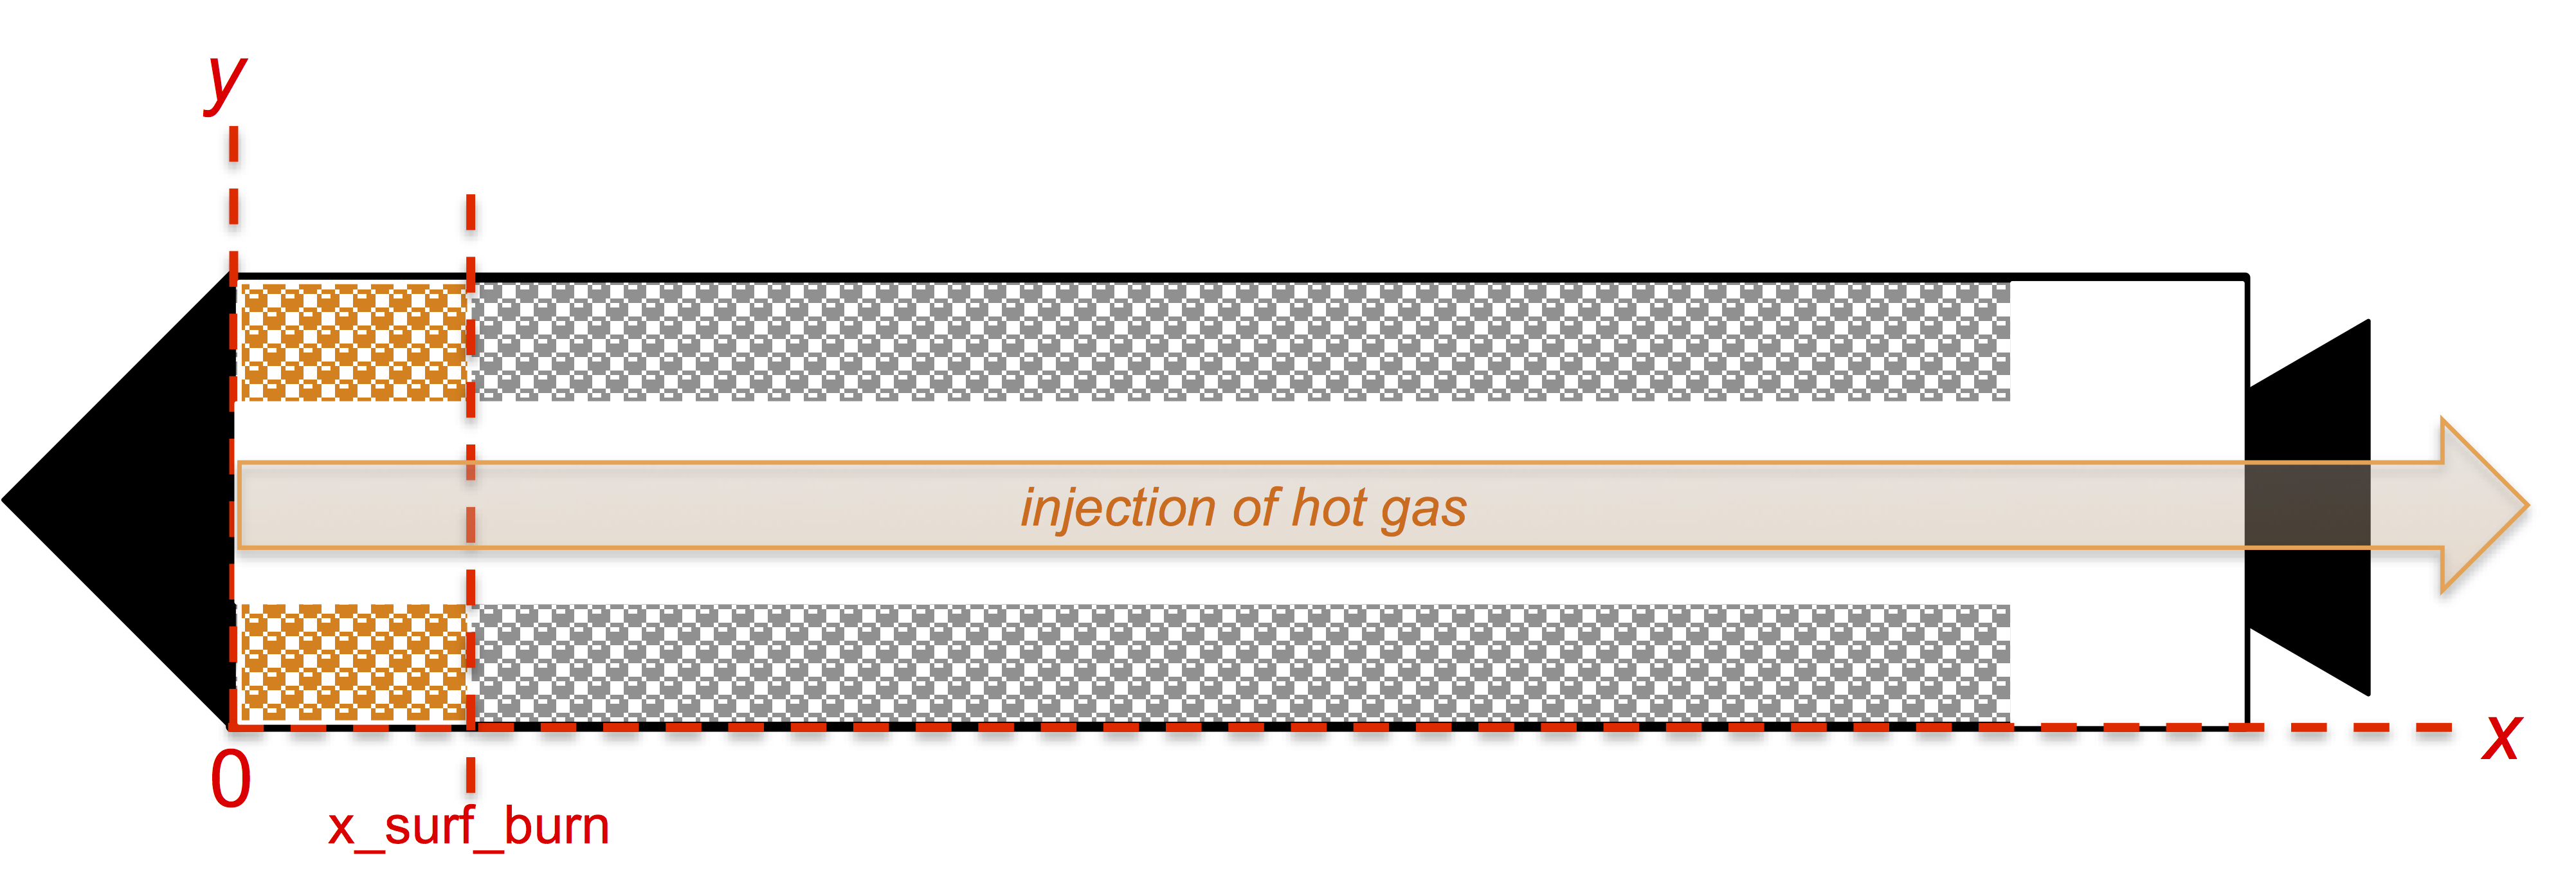
\includegraphics[width=0.9\textwidth]{../Figures/rocket.png}
\caption{Simple rocket. This schematic of a ``rocket'' illustrates the different regions, from the nozzle (far left), to the propellant (center), to the tail (far right). The variable \texttt{x\_surf\_burn} distinguishes between burning and non-burning propellant.}
\label{fig:rocket}
\end{figure}

\irref{Figure}{fig:rocket} shows a simple rocket with the nozzle at one end (left), the tail at the other (right), and the propellant in the middle. In the center of the chamber is a bore through which the gas escapes as the rocket (propellant) burns away. Depending on the situation, the propellant may or may not be burning at $t=0$ (orange vs gray propellant, respectively), and \texttt{x\_surf\_burn} (i.e., the value of $x$ that represents the burning surface) distinguishes between burning and non-burning propellant.

\irparanonum{film\_cons}{paramh} The input parameter \texttt{film\_cons} is somewhat misleading as it sounds like the film {\it coefficient}, $h$, such as in \irref{Section}{PreIgnit}. In actuality it is a combination of two constants.

\begin{equation}
{\cal C_{\rm film}} = \frac{h}{\lambda_c} = \frac{0.0287\rho_g U_\infty c_p}{\lambda_c}\left(x\rho_g U_\infty\mu_g c_p^2\over \lambda_g^2\right)^{-1/5}
\end{equation}

where $\lambda_c$ is the thermal conductivity of the solid. (See \ireq{eq}{eq:hfilmcoefffull}.) As illustrated in \irref{Section}{Setup}, \texttt{film\_cons} is used to calculate $g(T_s,T_g)$ in \ireq{eq}{eq:qc} and $\partial g/\partial T_s$ in \ireq{eq}{eq:qcprime}.

\irparanonum{ixsymm}{paramx} This parameter is a flag to enable or disable (axisymmetric) burning in cells at $t = 0$. This parameter can take on one of four values:

\begin{description}[labelindent=1.5cm]
\item[0]{No burning at $t$ = 0}
\item[1]{Burning along $x$-direction at $t = 0$}
\item[2]{Burning along $y$-direction at $t = 0$}
\item[3]{Burning along $z$-direction at $t = 0$}
\end{description}

\irparanonum{x\_surf\_burn}{paramb} This parameter is intimately tied to \texttt{ixsymm} as it specifies the width (or distance) of the propellant that is burning at $t=0$, such as that shown in \irref{Figure}{fig:rocket}. Note that if \texttt{ixsymm = 0}, then there is no propellant burning when the simulation begins (i.e., at $t=0$), and \texttt{x\_surf\_burn} is unused.

\irsssection{Divergence Boundaries}{DivBound}

\Rocburn\ will stop if the values for $P$, $T_{\rm flame}$ (i.e., $T_\star$), and $r_b$ fall outside of their user-specified ranges. 

\begin{itemize}
\item{$P_{\rm min} < P < P_{\rm max}$}
\item{$T_{\rm min} < T_\star < T_{\rm max}$}
\item{$r_{b,{\rm min}} < r_b < r_{b, {\rm max}}$}
\end{itemize}

There are old versions of the \Rocburn\ input file that did not require these ranges to be specified in the input file. If these old versions are used, \Rocburn\ will use internally set limits.

\begin{itemize}
\item{$\SI{1}{\kilo\pascal} < P < \SI{100}{\mega\pascal}$}
\item{$\SI{290}{\kelvin} < T_\star < \SI{10 000}{\kelvin}$}
\item{$\SIper{-1}{\nano\meter\per\second} < r_b < \SIper{100}{\meter\per\second}$}
\end{itemize}

\irsssection{Grid Parameters}{GridParams}

As discussed in the introduction to \irref{Section}{Code}, \Rocburn\ specifies a very thin temperature boundary layer associated with the heat wave traveling into the solid. More importantly this thin region requires a stretched grid to properly resolve the heat flux at the surface.

\irparanonum{igrid}{paramgrid} This parameter is a flag to select the type of computational grid used to represent this thin region. This parameter can take on one of two values:

\begin{description}[labelindent=1.5cm]
\item[1]{Exponential grid}
\item[2]{Boundary layer grid}
\end{description}

\irparanonum{xmax|numx}{paramxmax} This parameter specifies the width of this thin region, i.e., the width into propellant depth of interface. Note that \texttt{xmax} must be negative! In addition the density of points in this region is specified by \texttt{numx}, i.e., the maximum number of \texttt{xmax} grid points. These two parameters are intimately tied to \texttt{igrid}. If an exponential grid is selected, i.e., \texttt{igrid = 1}, there two parameters are unused.

\irparanonum{beta}{parambeta} As suggested above, the interface region requires a slightly different grid to properly resolve the heat flux at the surface. The grid parameters are scaled by the stretch constant \texttt{beta}.

\irsssection{Lookup Table Parameters}{TableParams}

As briefly touched upon in \irref{Section}{Intro} and again at the end of \irref{Section}{PostIgnit}, \Rocburn\ has a unique feature that allows for use of an externally calculated parameter table. This table is created by averaging the solid phase heat conduction over a plane that is parallel to the mean surface, accounting for the rotational terms that arise due to the uneven surface.

\irparanonum{TABUSE|TABNAM}{paramtab} The \texttt{TABUSE} parameter is a flag to enable or disable the use of an external table. This parameter can take on one of two values:

\begin{description}[labelindent=1cm]
\item[0]{Use analytical results to calculate properties and parameters (i.e., no table)}
\item[1]{Exercise the table algorithm portion of \Rocburn}
\end{description}

If \texttt{TABUSE = 1} \Rocburn\ will read in the information from a text file, the name of which is specified by \texttt{TABNAM}, e.g., \irfilename{RBRNtable.dat}. Note that if \texttt{TABUSE = 0}, \texttt{TABNAM} is unused.

\irssection{Working \Rocburn\ Input File}{Control}

A working example of the \Rocburn\ input file (\irfilename{RocburnPYControl.txt}) is shown below, i.e, the input parameters are in the correct order as required by \Rocburn. Note that the line numbers at the left of this sample file (e.g., 1, 2, 3, etc.) are \underline{{\bf not}} part of the input file; they are provided for ease of reference. (See \irref{Section}{Code}.)

\begin{small}
\begin{Verbatim}[frame=single]
                              RocburnPYControl.txt

 1   0.3912       a_p           in rb = a_p*(P/Pref)^n, rb in cm/sec & P in atm
 2   0.461        n_p           in rb = a_p*(P/Pref)^n, rb in cm/sec & P in atm
 3   34.0         Pref          in rb = a_p*(P/Pref)^n, atm
 4   180000.0     Ac            Condensed_phase_prefactor,(cm/s)
 5   24000.0      eg_ru         Gas phase activation temp, (K)
 6   12500.0      ec_ru         Solid phase activation temp, (K)
 7   1.00e-3      alfac         Solid phase thermal diffusivity, (cm^2/s)
 8   0.350        C             Specific heat (ga & condensed phases), (cal/g-K)
 9   2.00e-4      lamg          Gas phase thermal conductivity, (cal/cm-s-K)
10   1.0e-6       delt          Timestep, (s);_WATCH STABILITY
11   2            igrid         Grid control distribution; 1 = exp, 2 = bl
12   100          numx          number of points in propellant depth
13   -0.200       xmax          Maximum x location, (cm); MUST BE NEGATIVE!
14   1.010        beta          Grid stretching parameter,
15   2850.0       Tstar0        adiabatic flame temperature, Tstar0 (K)
16   300.0        To            cold temperature, To (K)
17   850.0        Tignition     ignition temperature, Tignition (K)
18   300.0        Tsurf         surface temperature
19   560.08d0     film_cons     constant in film coefficient [ W/ (m^2 K) ]
20   1            ixsymm        axisymmetric initial burning, use x_surf_burn
21   0.1815       x_surf_burn   last surface x location burning from the onset
22   1.d8         press_max     maximum pressure allowed to be passed in [Pa]
23   1.d2         press_min     minimum pressure allowed to be passed in [Pa]
24   1.d0         rb_max        maximum burn rate allowed [m/sec]
25   -1.d-6       rb_min        minimum burn rate allowed [m/sec]
26   1.d5         Tf_max        maximum gas temperature allowed [K]
27   100.00       Tf_min        minimum gas temperature allowed [K]
28   0            TABUSE        1 USE table algorithm, 0 USE analytical results
29   RBRNtab.dat  TABNAM        name of the file w/ table
\end{Verbatim}
\end{small}

\bibliographystyle{apa}
\bibliography{all_refs}

%\newpage

%\begin{appendix}
%\end{appendix}

%==================================================================
\end{document}